\chapter{Supplementary for Chapter 1}
\label{ch:SupplIntro}

\section{FASTQ format}\label{sec:fastq-format}

{\color[rgb]{0.447059,0.678431,0.274510}\verb!@ERR030856.1!}
{\color[rgb]{0.500000,0.500000,0.500000}\verb!HWI-BRUNOP16X_0001:1:1:2669:1073#0!}%
{\color[rgb]{1.000000,0.000000,0.000000}\verb!/1!}\\
\verb!AAAGGATTATGCAGANGTAGGGCGTGTNNNNNNNNNNNNNGGCTGGGGNNNNNNNNNNNNNNNNNNATNNNCTGACCANCTGAAGTATGTCANGCTGCCT!\\
{\color[rgb]{0.698039,0.145098,0.450980}+}\\
{\color[rgb]{0.000000,0.000000,0.555711}\verb!HHHHHHHIHHFFFFF#>>@>GGGFG###########################################################################!}\\
{\color[rgb]{0.447059,0.678431,0.274510}\verb!@ERR030856.2!}
{\color[rgb]{0.500000,0.500000,0.500000}\verb!HWI-BRUNOP16X_0001:1:1:4476:1072#0!}%
{\color[rgb]{1.000000,0.000000,0.000000}\verb!/1!}\\
\verb!GATAGATTATCAGAANGACAGTTACTTNNNNNNNNNNNNNGGGCACTTNNNNNNNNNNNNNNNNNNATNNNTCATAAGNNCTGTTGCCAAATNAGTGATA!\\
{\color[rgb]{0.698039,0.145098,0.450980}+}\\
{\color[rgb]{0.000000,0.000000,0.555711}\verb!HHHHHHHHHHDDDDD#@@AAGGGGG###########################################################################!}

{\footnotesize
Legende:\\
\quad{\color[rgb]{0.447059,0.678431,0.274510}\textbullet Read identifier}\\
\quad{\color[rgb]{0.500000,0.500000,0.500000}\textbullet Optional information (here flow cell lane:tile number:x:y:z)}\\
\quad{\color[rgb]{1.000000,0.000000,0.000000}\textbullet First member of pair (here) or single-end}\\
\quad\textbullet Nucleotide sequence of the read\\
\quad{\color[rgb]{0.698039,0.145098,0.450980}\textbullet Separator (+ or any string of character)}\\
\quad{\color[rgb]{0.000000,0.000000,0.555711}\textbullet Phred score (here Phred 33)}
}


\section{Phred score}\label{sec:PhredScore}

\begin{table}
\centering
\caption{Phred quality score to accuracy significance}
\label{PhredtoAccuracy}
\begin{tabular}{@{}lll@{}}
\toprule
\begin{tabular}[c]{@{}l@{}}Phred quality\\ score ($Q$)\end{tabular} & \begin{tabular}[c]{@{}l@{}}Probability of\\ incorrect\\ base call\end{tabular} & \begin{tabular}[c]{@{}l@{}}Base call\\ accuracy\end{tabular} \\ \midrule
10 & 1 in 10 & 90\% \\
20 & 1 in 100 & 99\% \\
30 & 1 in 1,000 & 99.9\% \\
40 & 1 in 10,000 & 99.99\% \\ \bottomrule
\end{tabular}
\end{table}

The \gls{Phred} quality score can be encoded in several standards.

\begin{verbatim}
SSSSSSSSSSSSSSSSSSSSSSSSSSSSSSSSSSSSSSSSS.....................................................
..........................XXXXXXXXXXXXXXXXXXXXXXXXXXXXXXXXXXXXXXXXXXXXXX......................
...............................IIIIIIIIIIIIIIIIIIIIIIIIIIIIIIIIIIIIIIIII......................
.................................JJJJJJJJJJJJJJJJJJJJJJJJJJJJJJJJJJJJJJJ......................
LLLLLLLLLLLLLLLLLLLLLLLLLLLLLLLLLLLLLLLLLL....................................................
!"#\$\%&'()*+,-./0123456789:;<=>?@ABCDEFGHIJKLMNOPQRSTUVWXYZ[\]^_`abcdefghijklmnopqrstuvwxyz{|}~
 |                         |    |        |                              |                     |
33                        59   64       73                            104                   126
 0........................26...31.......40
                          -5....0........9.............................40
                                0........9.............................40
                                   3.....9.............................40
 0........................26...31........41

S - Sanger        Phred+33,   cores des séquences brutes compris entre 0 et 40
X - Solexa        Phred+64, scores des séquences brutes compris entre -5 et 40
I - Illumina 1.3+ Phred+64,  scores des séquences brutes compris entre 0 et 40
J - Illumina 1.5+ Phred+64,  scores des séquences brutes compris entre 3 et 40
     avec 0=inutilisé, 1=inutilisé, 2=Indicateur de contrôle qualité de segment de séquence (en gras)
L - Illumina 1.8+ Phred+33,  scores des séquences brutes compris entre 0 et 41
\end{verbatim}

\begin{figure}
    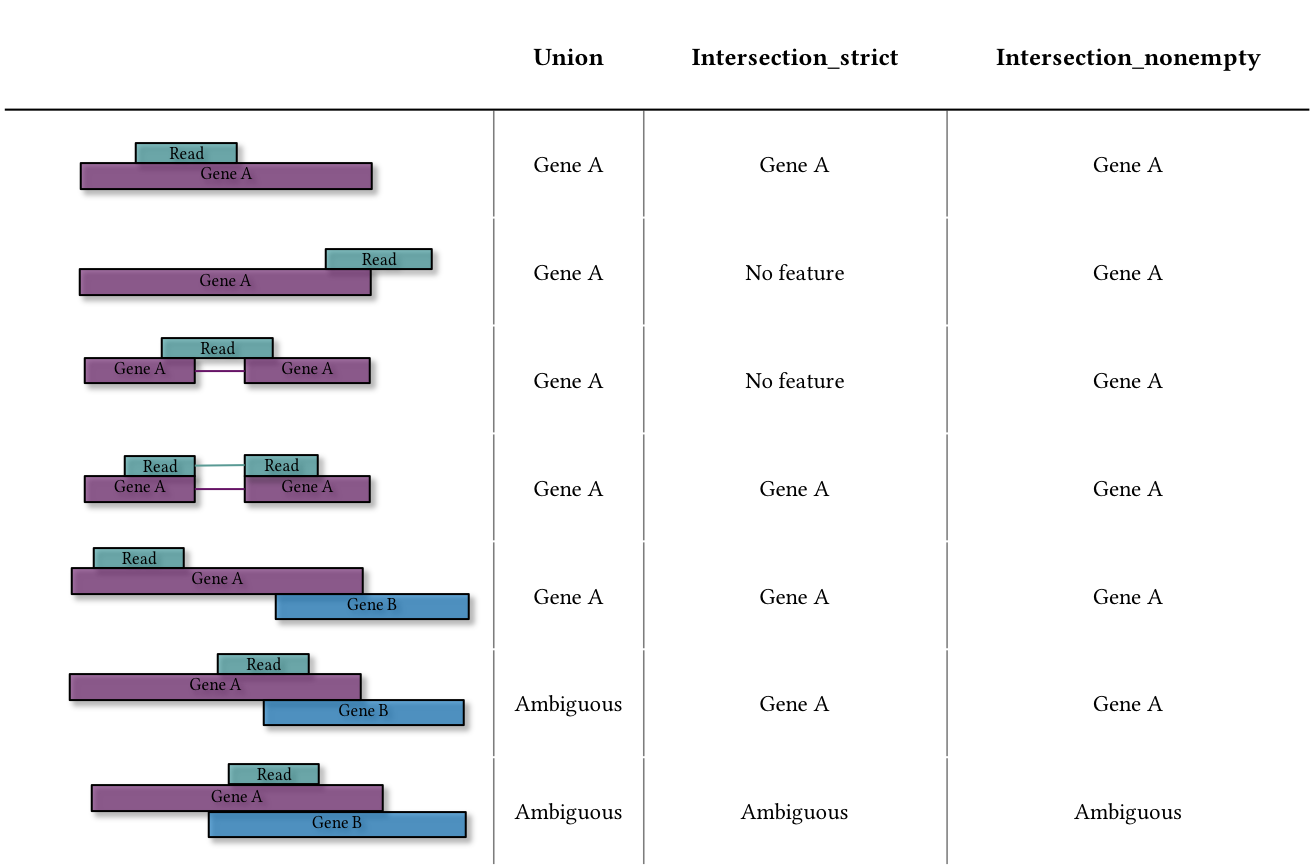
\includegraphics[scale=0.60]{introduction/interestHtseq}\centering
    \caption[Overlap resolution effects for each \htseq\
    mode]{\label{fig:htseqMode}\textbf{Overlap resolution effects for each \htseq\
    mode.} Each mode resolves a number of overlap situations differently. The
    mode used in this thesis is the \texttt{intersection non-empty} mode. This
    specific mode resolves more situations than the two others. Hence, the loss
    of ambiguous reads is lesser in this mode. [Adaptated from HTseq
    documentation: \footnotesize{\href{http://www-huber.embl.de/HTSeq/doc/count.html}%
    {http://www-huber.embl.de/HTSeq/doc/count.html}}]}
\end{figure}



\begin{table}[]
\centering
\caption{\gls{FPKM} are unsuitable for differential expression analysis}
\label{tab:noFPKM4DEA}
\begin{tabular}{@{}lcccc@{}}
\toprule
\multicolumn{1}{l|}{} & \multicolumn{2}{c|}{Sample 1} & \multicolumn{2}{c}{Sample 2} \\ \midrule
\multicolumn{1}{l|}{} & \multicolumn{1}{c|}{raw counts} & \multicolumn{1}{c|}{normalised counts} & \multicolumn{1}{c|}{raw counts} & normalised counts \\ \midrule
\multicolumn{1}{l|}{$Gene_{1}$} & \multicolumn{1}{c|}{100} & \multicolumn{1}{c|}{0.010} & \multicolumn{1}{c|}{80} & 0.008 \\
\multicolumn{1}{l|}{$Gene_{2}$} & \multicolumn{1}{c|}{100} & \multicolumn{1}{c|}{0.010} & \multicolumn{1}{c|}{80} & 0.008 \\
\multicolumn{1}{c}{\ldots} & \ldots & \ldots & \ldots & \ldots \\
\multicolumn{1}{l|}{$Gene_{i}$} & \multicolumn{1}{c|}{100} & \multicolumn{1}{c|}{0.010} & \multicolumn{1}{c|}{80} & 0.008 \\
\multicolumn{1}{l|}{$Gene_{i+1}$} & \multicolumn{1}{c|}{0} & \multicolumn{1}{c|}{0} & \multicolumn{1}{c|}{2000} & 0.2 \\ \midrule
\begin{tabular}[c]{@{}l@{}}Total number\\ of fragments ($F$)\end{tabular} & 10,000 & 1 & 10,000 & 1 \\ \bottomrule
\end{tabular}
\end{table}


\section{Isotopes of common elements and their natural
frequency}\label{app:isotopes}

\TK{Mettre en page et récuperer la biblio}
\begin{comment}
This table lists the mass and percent natural abundance for the stable nuclides. The mass of the longest lived
isotope is given for elements without a stable nuclide. Nuclides marked with an asterisk (*) in the abundance column
indicate that it is not present in nature or that a meaningful natural abundance cannot be given. The isotopic mass
data is from G. Audi, A. H. Wapstra Nucl. Phys A. 1993, 565, 1-65 and G. Audi, A. H. Wapstra Nucl. Phys A. 1995,
595, 409-480. The percent natural abundance data is from the 1997 report of the IUPAC Subcommittee for Isotopic
Abundance Measurements by K.J.R. Rosman, P.D.P. Taylor Pure Appl. Chem. 1999, 71, 1593-1607.
(trouver là : https://chemistry.sciences.ncsu.edu/msf/pdf/IsotopicMass_NaturalAbundance.pdf) 
\end{comment}

\begin{table}[]
\centering
\caption{Most common constitutive elements and their isotopes of proteins}
\label{tab:isotope}
\begin{tabular}{@{}clcr@{}}
\toprule
\begin{tabular}[c]{@{}c@{}}Z \\ (Atomic number)\end{tabular} &
    \multicolumn{1}{c}{Isotope} &
    \begin{tabular}[c]{@{}c@{}}Mass atomic\\ (u)\end{tabular} &
    \multicolumn{1}{c}{\begin{tabular}[c]{@{}c@{}}Natural frequency\\ (\%)\end{tabular}}\\
    \midrule
    1   & \isotope[1]{H}    & 1.007825  & 99.9885   \\
        & \isotope[2]{H}    & 2.014102  & 0.0115    \\
        & \isotope[3]{H}    & 3.016049  & *         \\
    6   & \isotope[12]{C}   & 12.000000 & 98.93     \\
        & \isotope[13]{C}   & 13.003355 & 1.07      \\
        & \isotope[14]{C}   & 14.003242 & *         \\
    7   & \isotope[14]{N}   & 14.003074 & 99.632    \\
        & \isotope[15]{N}   & 15.000109 & 0.368     \\
    8   & \isotope[16]{O}   & 15.994915 & 99.757    \\
        & \isotope[17]{O}   & 16.999132 & 0.038     \\
        & \isotope[18]{O}   & 17.999160 & 0.205     \\
    \bottomrule
\end{tabular}
\end{table}

